\documentclass[aspectratio=169]{beamer}
%
% Choose how your presentation looks.
%
% For more themes, color themes and font themes, see:
% http://deic.uab.es/~iblanes/beamer_gallery/index_by_theme.html
%
\mode<presentation>
{
  \usetheme{default}      % or try Darmstadt, Madrid, Warsaw, ...
  \usecolortheme{default} % or try albatross, beaver, crane, ...
  \usefonttheme{default}  % or try serif, structurebold, ...
  \setbeamertemplate{navigation symbols}{}
  \setbeamertemplate{caption}[numbered]
} 

% Set background to black and text to white
\setbeamercolor{background canvas}{bg=black}
\setbeamercolor{normal text}{fg=white}
\setbeamercolor{frametitle}{fg=white}
\setbeamercolor{title}{fg=white}

% You can continue to set other colors as needed:
\setbeamercolor{item}{fg=magenta} % Color of bullets
\setbeamercolor{subitem}{fg=yellow}
\setbeamercolor{subsubitem}{fg=cyan}
% ...
\setbeamertemplate{frametitle}[default][center]

\usepackage[english]{babel}
\usepackage[utf8]{inputenc}
\usepackage[T1]{fontenc}
\usepackage{graphicx}

% Set larger font for frame title
\setbeamerfont{frametitle}{size=\huge}

\usepackage{emoji}

\begin{document}

\begin{frame}{GPU architecture basics}
\begin{columns}[T]
    \begin{column}[T]{0.5\textwidth}
    Triton abstracts away many low-level details of how GPUs work so that you don't have to think about them \\
    \vspace{0.1in}
    This lesson is just a rough primer; do not feel like you need to understand the specifics of each diagram. It'll make more sense when we start coding
    \end{column}
    \begin{column}{0.5\textwidth}
        
\includegraphics[height=0.8\textheight]{pics/triton-logo.png}
    \end{column}
\end{columns}
\end{frame}

\begin{frame}{CPU vs GPU}
\centering
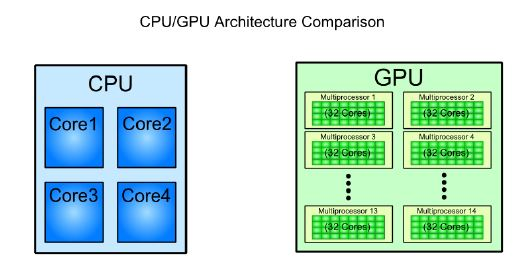
\includegraphics[width=0.8\textwidth]{pics/architecture_comparison-2717927587.jpg}
\end{frame}

\begin{frame}{memory hierarchy}
\centering
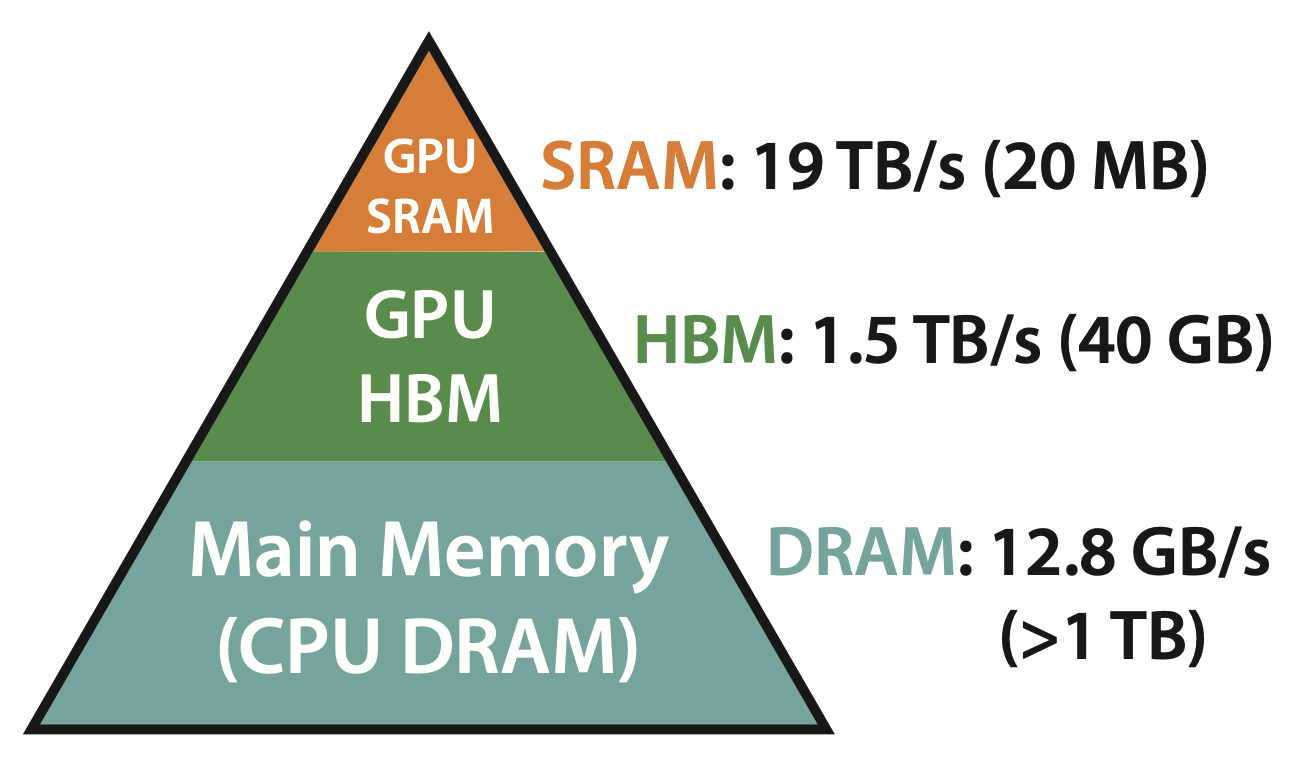
\includegraphics[width=0.8\textwidth]{pics/mem_hierarchy.png}
\end{frame}

\begin{frame}{one streaming multi-processor (SM) per pool of SRAM}
\centering
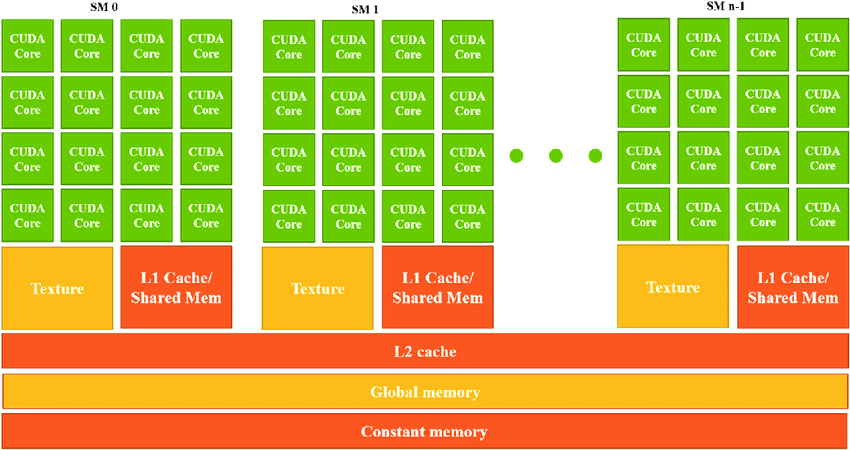
\includegraphics[width=0.8\textwidth]{pics/SM.png}
\end{frame}

\begin{frame}{programs}
\vspace{-0.5in}
a program is a specific instance of our kernel code run in parallel alongside many others. It is differentiated from other programs by the chunk of data it is assigned to work on
\begin{itemize}
    \item each program is defined by a program ID (PID) which is a tuple full of integers
    \begin{itemize}
        \item we use this PID alongside indexing logic to figure out which chunk of a tensor the program works on
    \end{itemize}
    \item at least one program is called per SM, depending on how many can fit
        \begin{itemize}
            \item number of PIDs per SM = amount of SRAM // SRAM required per PID
        \end{itemize}
    \item if your code requires more data per single program than fits within the SM's pool of SRAM, it'll error
    \item If different PIDs in the same SM load the same data, then they'll share rather than loading \& storing duplicates (we will take advantage of this)
\end{itemize}
\end{frame}

\begin{frame}{cores \& warps}
\vspace{-0.5in}
A core is the smallest unit of compute; it performs the actual floating point operations
\begin{itemize}
    \item unlike CPU cores, GPU cores cannot do any arbitrary operation; they're built primarily for FLOPs
    \item one GPU core performs one FLOP at a time
\end{itemize}
A warp is the smallest grouping of GPU cores
\begin{itemize}
    \item 32 cores per warp on Nvidia; 64 on AMD
    \item all cores in a warp must perform the exact same operation
    \item there are multiple warps per PID; you don't have to worry about how many
\end{itemize}
\end{frame}

\end{document}